
Fat Finger is an application that operates on a standard Apple iPad mini with retina display device, which runs the iOS 7 (version 7.1.1) operating system. The device has the following specifications:


\begin{table}[H]
\centering
\begin{tabular}{l || l }
Specification & Description \\
\hline
Display & 7.9-inch (diagonal) LED-back-lit Multi-Touch \\
Display resolution & 2048-by-1536 resolution at 326 ppi
\\
Chip: & A7 chip with 64-bit architecture
\end{tabular}
\caption{Apple iPad mini with Retina Display Characteristics}
\label{tab:ipadspecs}
\end{table}


Fat Finger can also be ported on any other iPad devices that run iOS version 7 or higher of the Apple's mobile operating system (iOS). It should be mentioned that while iPad devices come in different screen sizes and resolutions, porting an App from one device to another is not an issue anymore. This is mainly feasible due to the innovative way of thinking in terms of pixels and points, Apple proposed for using graphics on an iOS device. 

% [reference: http://codeatuts.blogspot.ch/2012/11/interlude-13-pixels-vs-points-in-ios.html]

In particular, since iOS 4, dimensions are measured in \textbf{“points”} instead of pixels. All coordinate values and distances are specified using points, which are floating-point values. One point can refer to one or more pixels. The measurable size of a point varies from device to device and is largely irrelevant. Points provide a fixed frame of reference for drawing graphics on screen. To have an inside look on how points correspond to pixels, imagine that an iPad screen 768 x 1024 points and is size independent. Thus, this point resolution scales to the following pixel resolution for some referential models:


\begin{itemize}
    \item \textbf{iPad 1} - 768 x 1024 pixels (scale factor of 1.0)
    \item \textbf{iPad Air} - 1536 x 2048 pixels (scale factor of 2.0)
    \item \textbf{iPad Mini - Retina Display} - 1536 x 2048 pixels (scale factor of 2.0)
 \end{itemize}

When performing graphical operations, you should specify your measurements in points for all devices, and iOS automatically draws everything to the right proportion on the screen.  The outcome is that when you draw the same content on two similar devices, it has the same scale on both. 

The   code   has   been   developed in Objective C language using Xcode. Xcode is an Integrated Development Environment (IDE)  created by Apple for developing software for both OS X and iOS. Full Documentation for developing iOS applications is also included, alongside with many other utilities that are designed to enhance your coding experience (Tester, Debugger, etc.). Apple along with the release of iOS 8, last June, also released a new programming language for coding Apple software, \textbf{Swift}.

\emph{"Swift is a multi-paradigm, compiled programming language created by Apple for iOS and OS X development. Introduced at Apple's 2014 Worldwide Developers Conference, Swift is designed to work with Apple's Cocoa and Cocoa Touch frameworks and the large body of existing Objective-C code written for Apple products. Swift is intended to be more resilient to erroneous code ("safer") than Objective-C. It is built with the LLVM compiler included in Xcode 6, and uses the Objective-C runtime, allowing C, Objective-C, Objective-C++ and Swift code to run within a single program."} \cite{wikiSwift}












%%%%%%%%%%%%%%%%%%%%%%%%%%%%%
%%%%%%%%%%%%%%%%%%%%%%%%%%%%%
%%%%%%%%%%%%%%%%%%%%%%%%%%%%%
%%%%%%%%%%%%%%%%%%%%%%%%%%%%%
%%%%%%%%%%%%%%%%%%%%%%%%%%%%%
%%%%%%%%%%%%%%%%%%%%%%%%%%%%%
\section{Fat Finger Application Description}


Fat Finger is an application which has been built to test the capabilities and the limits of the index finger's operational skills, on using the contact area touching the screen for integrating with a mobile device. The interaction with the finger requires an interface that will always listen to touch events on the screen. Thus, Fat Finger, whilst not being a complete application, it embeds all the infrastructure needed to support the new interaction we are proposing. The basic scenario is the following:
 \emph{Whenever a finger is touching the screen we should be able to calculate the contact area between the finger and the screen.} After obtaining that raw data, we should use that to interact with the interface provided. Despite how simple it may seem at a first glance, Apple does not provide a way to calculate this contact area, and neither does with the shape of the area covered by the finger. The iPad’s API only provides the major radius in pixels of a contact points' ellipse, which can be in rough lines obtained as follows:



\begin{lstlisting}
	NSValue *val = [touch valueForKey:``_pathMajorRadius''];
 	float size = [val floatValue]; //size in pixels
\end{lstlisting}


As a result, we can obtain only the major radius of the area covered by the finger. Moreover, we can not have continuous observation of the area but we can calculate this size only when a new touch event has happened. Generally in iOS, touch is event driven. Whenever a finger is touching the screen a relevant function is triggered to serve this event. iOS provides us the following 4 basic functions for handling touch events:

\begin{itemize}
	\item \textbf{TouchesBegan} – This is called when the screen is first touched.

	\item \textbf{TouchesMoved} – This is called when the location of the touch changes as the user is sliding their fingers around the screen.

	\item \textbf{TouchesEnded} – TouchesEnded is called when the users' fingers are lifted off the screen. 

	\item \textbf{TouchesCancelled} - It is called if the system cancels the sequence of touch events.
\end{itemize}	
	
Thus, whenever each of the first three functions are getting called, we can measure the size of the area covered by the finger. The problem arises exactly when we realize that each of the above functions is called when the location of the touch changes, and not when the contact area changes. In other words, a new event is triggered only when the center point of the touching area changes. Indeed, there are occasions that the contact area is changing without alternating the center of the ellipsis. 
 It results in non continuous observation of the contact area touching the screen, and there is not an existing way of alternating this behaviour ourselves. We are constrained in measuring the area if the location of the finger has been changed. Changes in contact area that do not alter the location in the screen, can not be measured. However, after investigation we realized that this circumstances are extremely rare under normal use so, despite the limitations we faced, our methodology works fine.


\subsection{Basic WorkFlow}
 
 Fat Finger application can be divided on the following modules:

 \begin{itemize}
\item \textbf{Start App} - Represents the launching of the application. 
\item \textbf{Register Participant} - In this module, we assign a new unique ID to each participant through a custom form.
\item \textbf{Calibrate} - Participant can calibrate his finger.
\item \textbf{Visualize} - Participant can visualize the previously obtained calibrated values. If he is not satisfied with the outcome, he can jump back to Calibration mode and calibrate again.
\item \textbf{Trials - Experiment} - This is the main part of the experiment, in which all trials are included.
\item \textbf{End of Experiment} - After having finished the experiment trials, experiment is finished.
 \end{itemize}

 The flowchart of those modules can be observed on Figure \ref{fig:FFBasicFlow}. We notice that there is a circular connection between Calibrate \& Visualize. This is due to the fact that we can calibrate and then visualize as many times as we need or want to. When we are satisfied with the calibrated values, we may proceed to the Experiment Trials. 

 \begin{figure}[h]
\centering
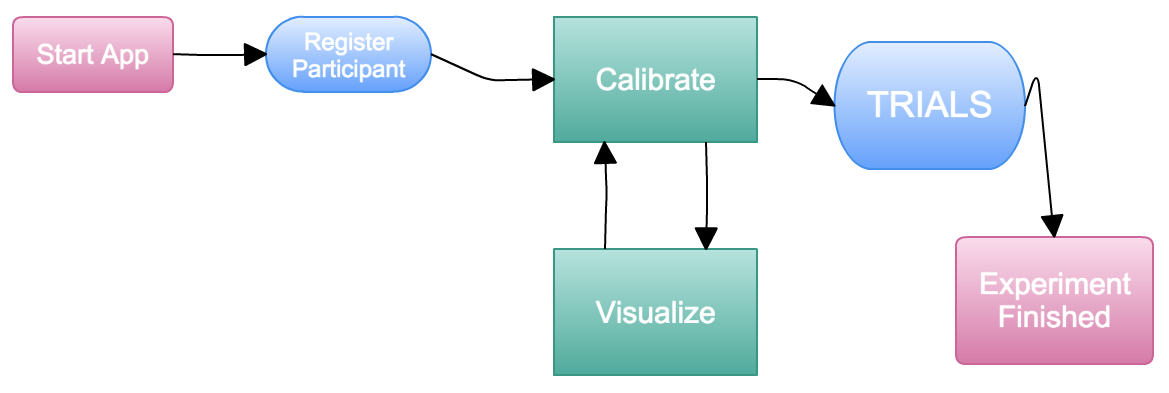
\includegraphics[width=\textwidth]{figures/FFBasicFlow.png}
\caption{Fat Finger - Abstract Flowchart of Basic Modules}
\label{fig:FFBasicFlow}
\end{figure}


%%%%%%%%%%%%%%%%%%%%%%%%%%%%%
%%%%%%%%%%%%%%%%%%%%%%%%%%%%%
%%%%%%%%%%%%%%%%%%%%%%%%%%%%%
%%%%%%%%%%%%%%%%%%%%%%%%%%%%%
%%%%%%%%%%%%%%%%%%%%%%%%%%%%%
%%%%%%%%%%%%%%%%%%%%%%%%%%%%%
\subsection{Basic Design of a Trial}
Each Trial has one basic design and interface. Our target was to find the most obvious and physical way to be able to on-screen present all the aspects we wanted. I ended up on using the design, illustrated in Figure \ref{fig:FFBasicTrialInterface}. The challenging part was in finding a competitive alternative to the simple bar design. The basic usage scenario is:

\emph{The user should move his finger, in a way to alternate the contact area between the screen and his finger. There should be an indicator that will give him feedback. He should know the amount of pressure his is applying to the screen, through a visual representation.}



 \begin{figure}[h]
\centering
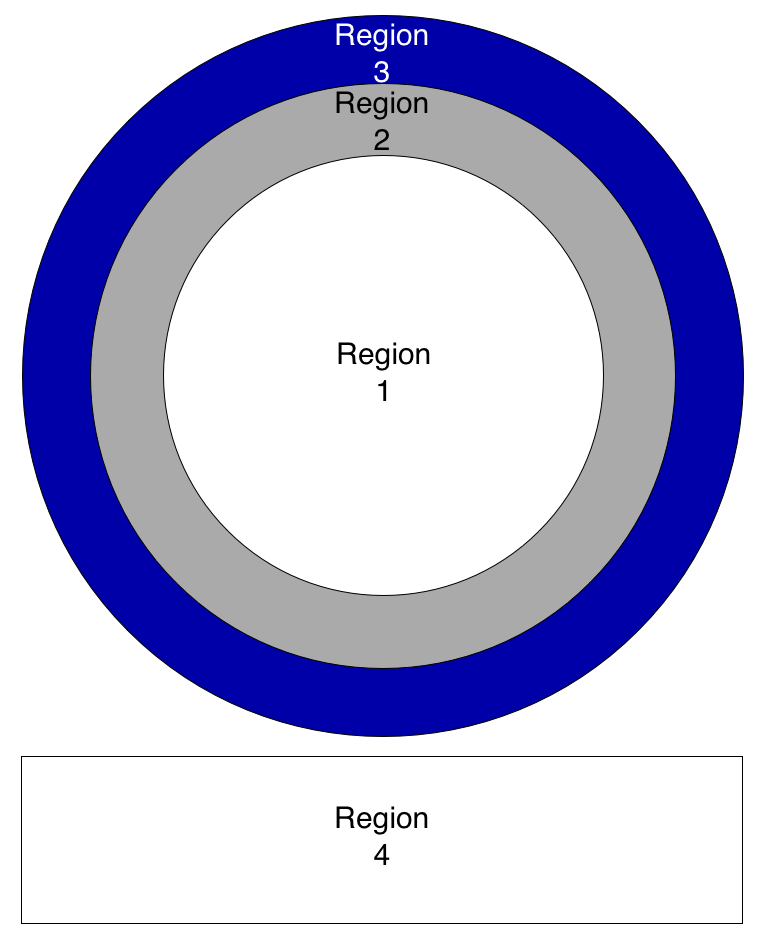
\includegraphics[scale=0.3]{figures/FFBasicTrialInterface.png}
\caption{Fat Finger - Basic Trial Interface}
\label{fig:FFBasicTrialInterface}
\end{figure}

In Figure \ref{fig:FFBasicTrialInterface} we can observe that our interface has 4 regions, all of them are placed on an iPad screen, and that the whole interface is based on overlapping circles with common center. Table \ref{tab:ffRegions} illustrates the correspondence between Numbers and regions.

\begin{table}[h]
\centering
\begin{tabular}{l || l }
Region No & Description \\
\hline
1 &  Non interactive region. Is placed there, simply in terms of design.\\
2 &  Red coloured targets are placed here.\\
3 &  FeedBack region.\\
4 &  Touch Region. Touch is enabled everywhere though.
\end{tabular}
\caption{Fat Finger - Basic Interface Regions}
\label{tab:ffRegions}
\end{table}

To better assimilate this design lets use a driving example. \emph{Imagine that there is a bar (similar to a progress bar), which is empty when we are barely touching the screen and full when we apply full pressure on the screen. Moreover in each trial, our mission is to achieve a specific level of filling it (e.g. 40\%). Since the bar depicts the movement of our finger, this can be achieved by alternating the area covered by our finger}. 

Now we are ready to move to the next level. Instead of familiarizing with this simple and purely designed idea, I decided to use the circle as the fundamental design shape. Region 3 (Table \ref{tab:ffRegions}) will be alternated while the participant is moving his finger, so as to perfectly map his movement. Therefore, we will have a partially filled circle for the different contact areas (Figure \ref{fig:FFPartlyFilled}).

 \begin{figure}[h]
\centering
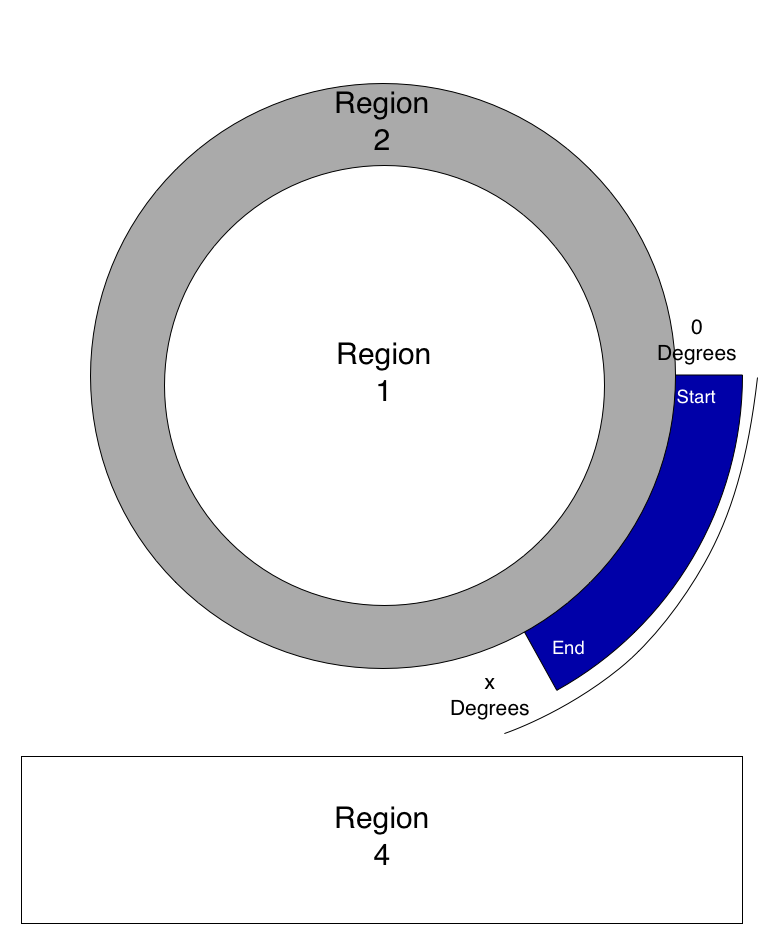
\includegraphics[scale=0.3]{figures/FFPartlyFilled.png}
\caption{Fat Finger - Basic interface during operation}
\label{fig:FFPartlyFilled}
\end{figure}

From Figure \ref{fig:FFPartlyFilled} we can point out many significant characteristics for our design. The starting point of measurement is x-positive axis, and degrees grow with a clockwise orientation. Thus when the contact area is minimum $x=0$, when maximum $x=360$ and $0<x<360$ for all other values. Finally there is a linear correspondence between contact size and degrees $x$, which is calculated through the type: $x = \frac{currentSize - minSize}{maxSize - minSize} * 360$, in degrees.













%%%%%%%%%%%%%%%%%%%%%%%%%%%%%
%%%%%%%%%%%%%%%%%%%%%%%%%%%%%
%%%%%%%%%%%%%%%%%%%%%%%%%%%%%
%%%%%%%%%%%%%%%%%%%%%%%%%%%%%
%%%%%%%%%%%%%%%%%%%%%%%%%%%%%
%%%%%%%%%%%%%%%%%%%%%%%%%%%%%
\section{Trial Categories}

% This section is devoted to present the different Trial categories that are encountered on Fat Finger.
Fat Finger consist of four (4) Trial categories. Those 4 categories are based on the values of 2 binary variables \textbf{TARGET \& FEEDBACK}. The values of this variables can be:
\begin{itemize}
	\item \textbf{Target} = \textbf{Discrete} or \textbf{Continuous}
	\item \textbf{Feedback} = be \textbf{Feedback} or \textbf{No Feedback}
\end{itemize}

Producing all possible combinations of values from \textbf{Target} and \textbf{Feedback} we end up having the 4 types we have already mentioned. All possible trials one can encountered belong to one of the those types, which are:


\begin{table}[H]
\centering
\begin{tabular}{l || l | l}
Targeting & Feedback & No Feedback \\
\hline \hline
Discrete & Feedback \& Discrete &  No Feedback \& Discrete\\
Continuous & Feedback \& Continuous & No Feedback \& Continuous
\end{tabular}
\caption{Fat Finger - Trial Categories}
\label{tab:ffTrialCateg}
\end{table}

During the experiment, those 4 types (Table \ref{tab:ffTrialCateg}) will occur multiple times with different variable difficulties. Difficulty can be defined as \emph{"The combination of the position and the size - width of the target"}. The smaller the target the more difficult one trial is. To be able to measure the difficulty of each Trial we use a new variable \textbf{N} which indicates how many buckets each trial has. So First we need to define what a bucket is.

\emph{Bucket is a part of the targets region (Region 2 in Figure \ref{fig:FFBasicTrialInterface}).The target region can be divided in N equal parts. Each of those parts is called Bucket. For example if $N=2$ then the first bucket is the "down" semicircle of the target region ($0-180$ degrees), and the second is the "upper" one ($180-360$ degrees)}

\textbf{N} varies inversely as the value of \textbf{Buckets}. In an inverse variation, the values of the two variables change in an opposite manner - as one value decreases, the other increases. Therefore, as N increases, the range of each bucket decreases. Moreover the ranges of all buckets should add up to 360 degrees. 

At this point, the values for the two basic variables \textbf{Target} and \textbf{Feedback} will be thoroughly analyzed.



%%%%%%%%%%%%%%%%%%%%%%%%%%%%%%%%%%%%
%%%%%%%%%%%%%%%%%%%%%%%%%%%%%%%%%%%% 
%% Explain the value of each variable

\begin{itemize}
	\item \textbf{Discrete}. This only relates to Region 2 (Figure \ref{fig:FFBasicTrialInterface}), so the formatting of the targets. In this type, targets are discrete, meaning that Region 2 is divided in N buckets, but only one of them is activated. The activated bucket is coloured in red and acts as the target for this trial. All other inactive buckets are coloured in gray. 

	\item \textbf{Continuous}. This also relates to Region 2 (Figure \ref{fig:FFBasicTrialInterface}) exclusively. In this type, Region 2 is not divided into buckets; at least visible ones. We think in term of targets, but we do not present them graphically. The target is just one small red line (a bucket with 1 degree range). However it might be impossible for the user to select such a tiny target, so we offer an offset area which is delimited with two yellow lines. The position of the target is not random. As I mentioned before, we still think in term of buckets. But instead of considering the whole bucket as a target, we just randomly select a small region inside that bucket, and draw the red line there. Thus, we have the same amount of trials as in the Discrete type.

	\item \textbf{Feedback} is related with Region 3 (Figure \ref{fig:FFBasicTrialInterface}). In this type, Region 3 is visible, meaning that we have continuous feedback while we are moving our finger. In order to select a target the user has to perform the Dwell technique. Thus, keep the edge of the blue line (Region 3) inside the red bucket for at least one second. Then a short sound confirms the selection and the trial is dismissed. Summarizing, the mission is: 

	\emph{Keep the edge of the blue "line" inside the red target for 1 second}.

	\item \textbf{No FeedBack} is also related with region 3 (Figure \ref{fig:FFBasicTrialInterface}). In this type, Region 3 is now invisible. Therefore we do not have feedback indicator while we are alternating the contact area between our finger and the screen. Thus we need to memorize the movement and be able to predict the position of the edge of the "blue" region. To confirm selection, user has to lift his finger from the screen, or perform the QuickRelease selection technique. The software will then choose the last contact area size,  before the lift as the one the user implied. As a consequence we can only lift the finger once. We are not allowed to perform retouches, because on the first lift, target selection will be performed. 

	It should also be mentioned that, in this type of trials, we are not forced to hit the target successfully. We just make a prediction and then lift our hand. Our input will be recorded and then displayed to us through a graphical Confirmation Interface.  Summarizing, in this type, our mission is:

	\emph{Touch the screen, alternate the contact area and make a prediction on where the blue line should be to hit the target, lift the finger when you are on the preferred contact size, and finally observe the outcome - feedback}.
\end{itemize}

We have now explained, and introduced all the necessary background, and we are ready to present the interface of the 4 categories of trials, as stated in Table \ref{tab:ffTrialCateg}.

%%%%%%%%%%%%%%%%%%%%%
%%%%%%%%%%%%%%%%%%%%%
%%%%%%%%%%%%%%%%%%%%%

\subsection{Feedback \& Discrete Targeting}


In this type of trials, we can understand that the targets will be discrete and there feedback on our input will be provided too. Figure \ref{fig:FD} presents the interface of this type. As we can see both Region 2 and 3 (Figure \ref{fig:FFBasicTrialInterface}) exist. Since we have \emph{Discrete} targets, Region 2 is separated in $n$ buckets, all with equal size. The target is the one coloured in red, and all others are inactive and coloured in gray. On the other hand, \emph{Feedback} keyword is mentioned too, which means that the blue circle (Region 3) exists. The movement of the blue region corresponds to the movement of our hand. To accomplish this trial, the participant needs to perform the Dwell selection technique.

\begin{figure}[H]
\centering
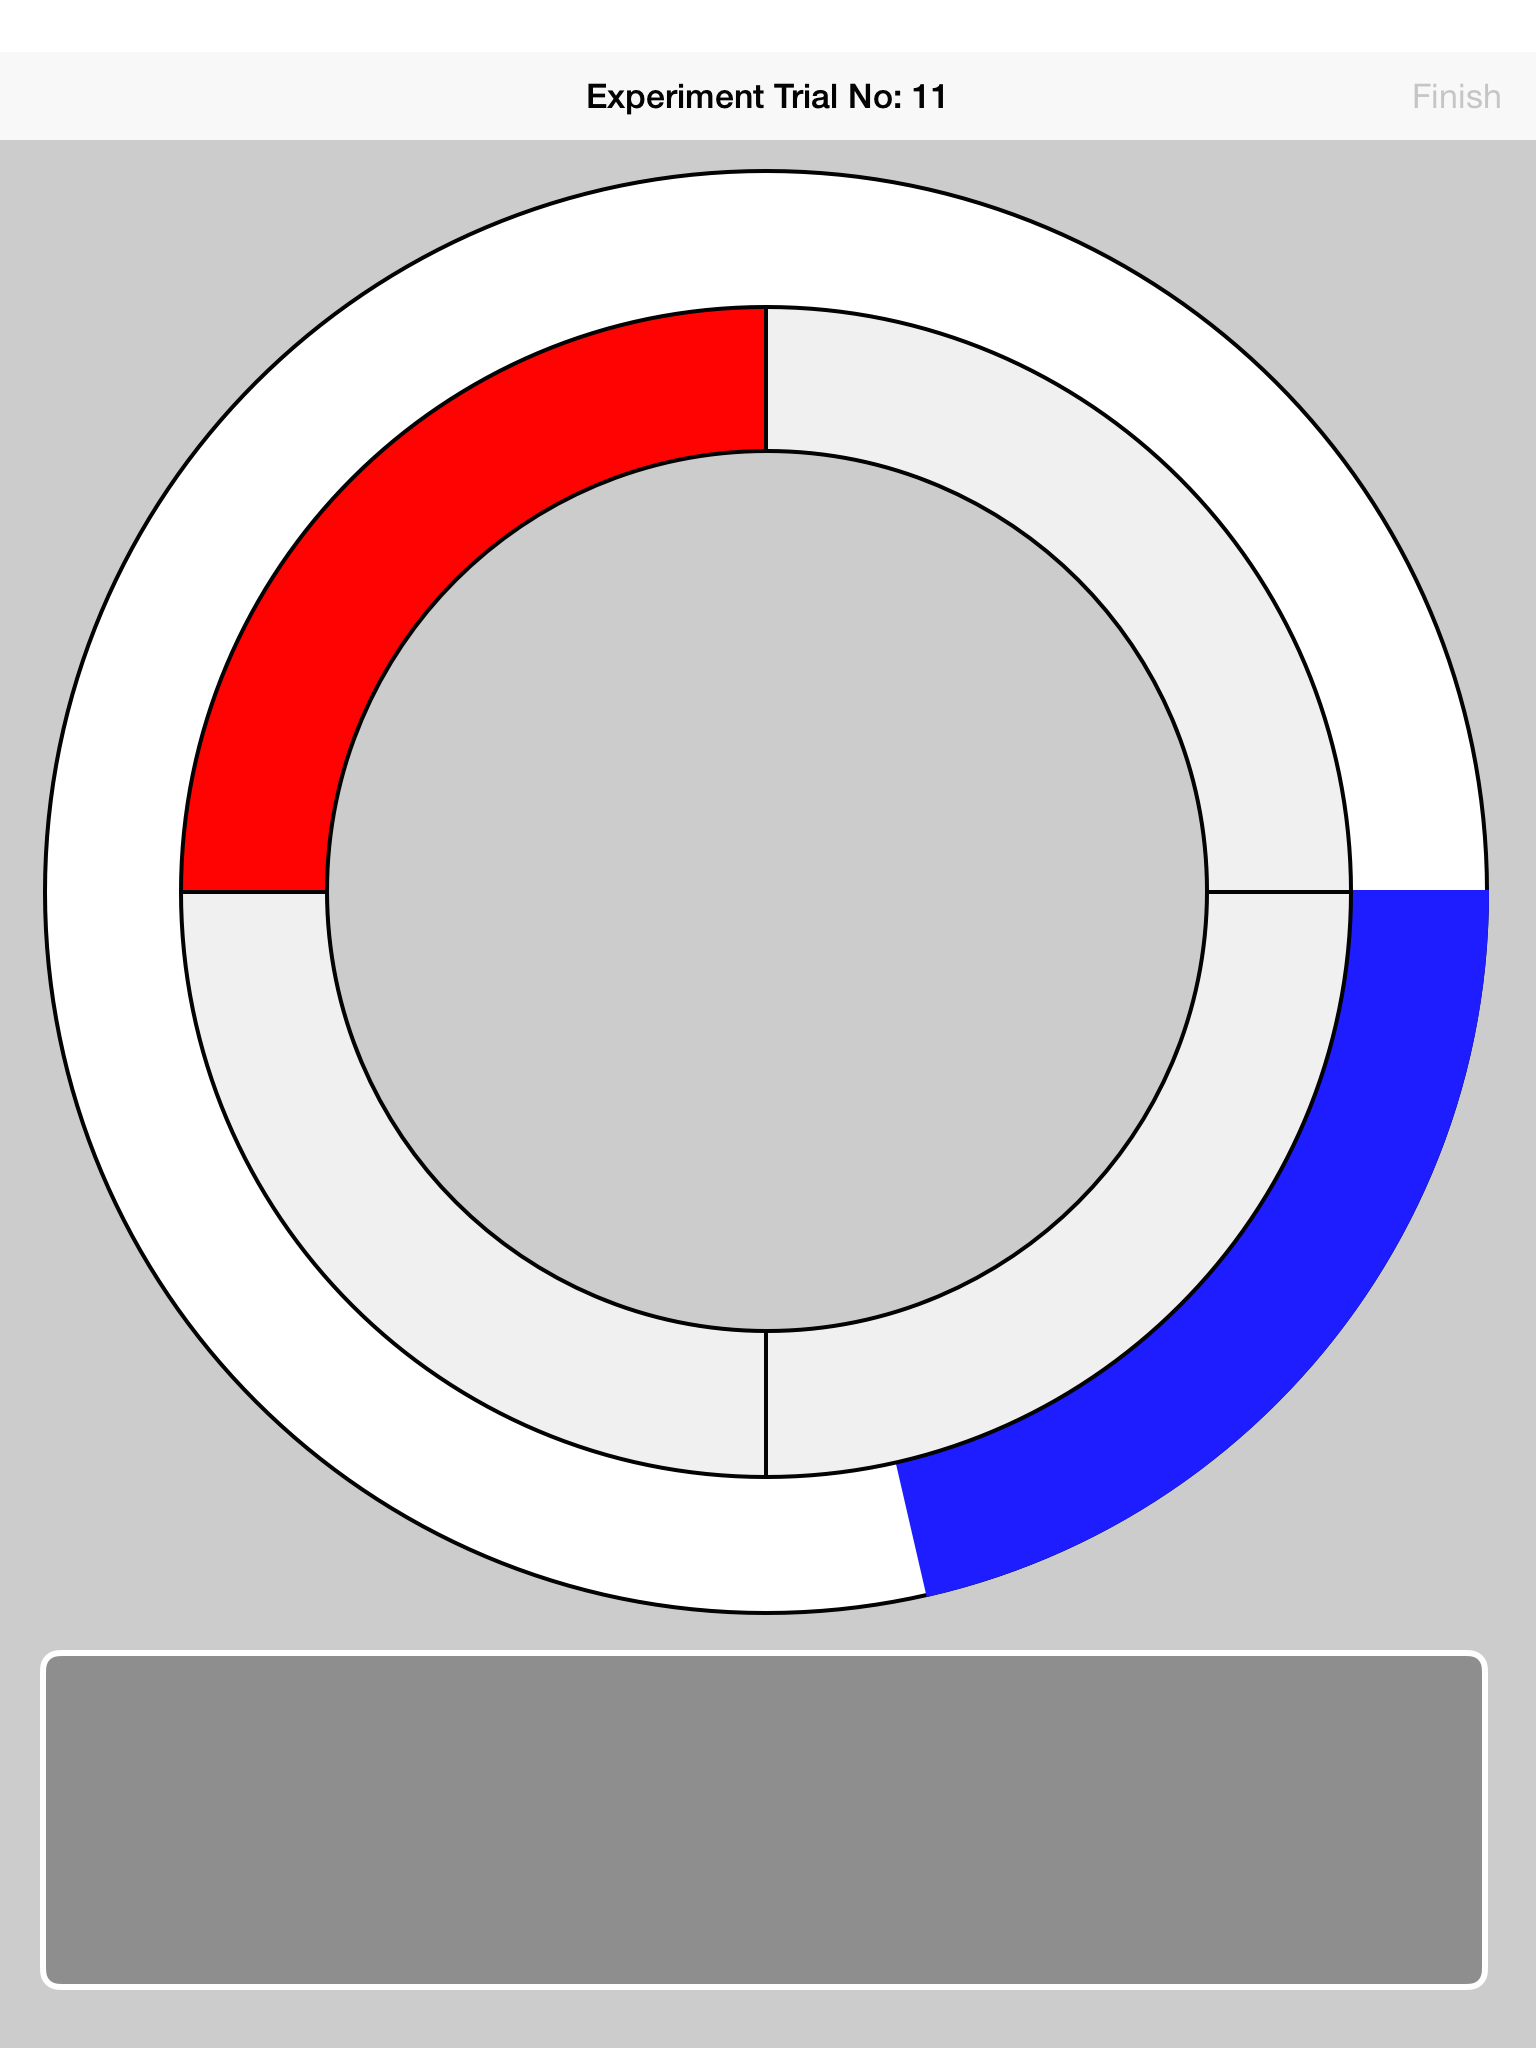
\includegraphics[scale=0.07]{figures/FD.png}
\caption{Feedback \& Discrete Targeting Interface}
\label{fig:FD}
\end{figure}


%%%%%%%%%%%%%%%%%%%%%
%%%%%%%%%%%%%%%%%%%%%
%%%%%%%%%%%%%%%%%%%%%

\subsection{Feedback \& Continuous Targeting}

In this occasion, we are still provided with feedback on our input, but the target will now be of type Continuous. Figure \ref{fig:FND} presents the interface of this category. \emph{Continuous} targets mean that only one thin red line exist in Region 2 (Figure \ref{fig:FFBasicTrialInterface}). While the position of the target is related with buckets, the actual buckets are just invisible. As we previously mentioned, the red line is randomly positioned within one of the N buckets. The two yellow lines, surrounding the red one are the offset limits and their distance is the offset range.  User can confirm a target by staying inside that range, however he is instructed to target as close and accurate to the target as possible. Finally, \emph{Feedback} keyword specifies that Region 3 exists. The process for confirming the selection of a target, is to keep the moving edge of the blue region inside the range of the target (yellow lines), for at least 1 second.

\begin{figure}[H]
\centering
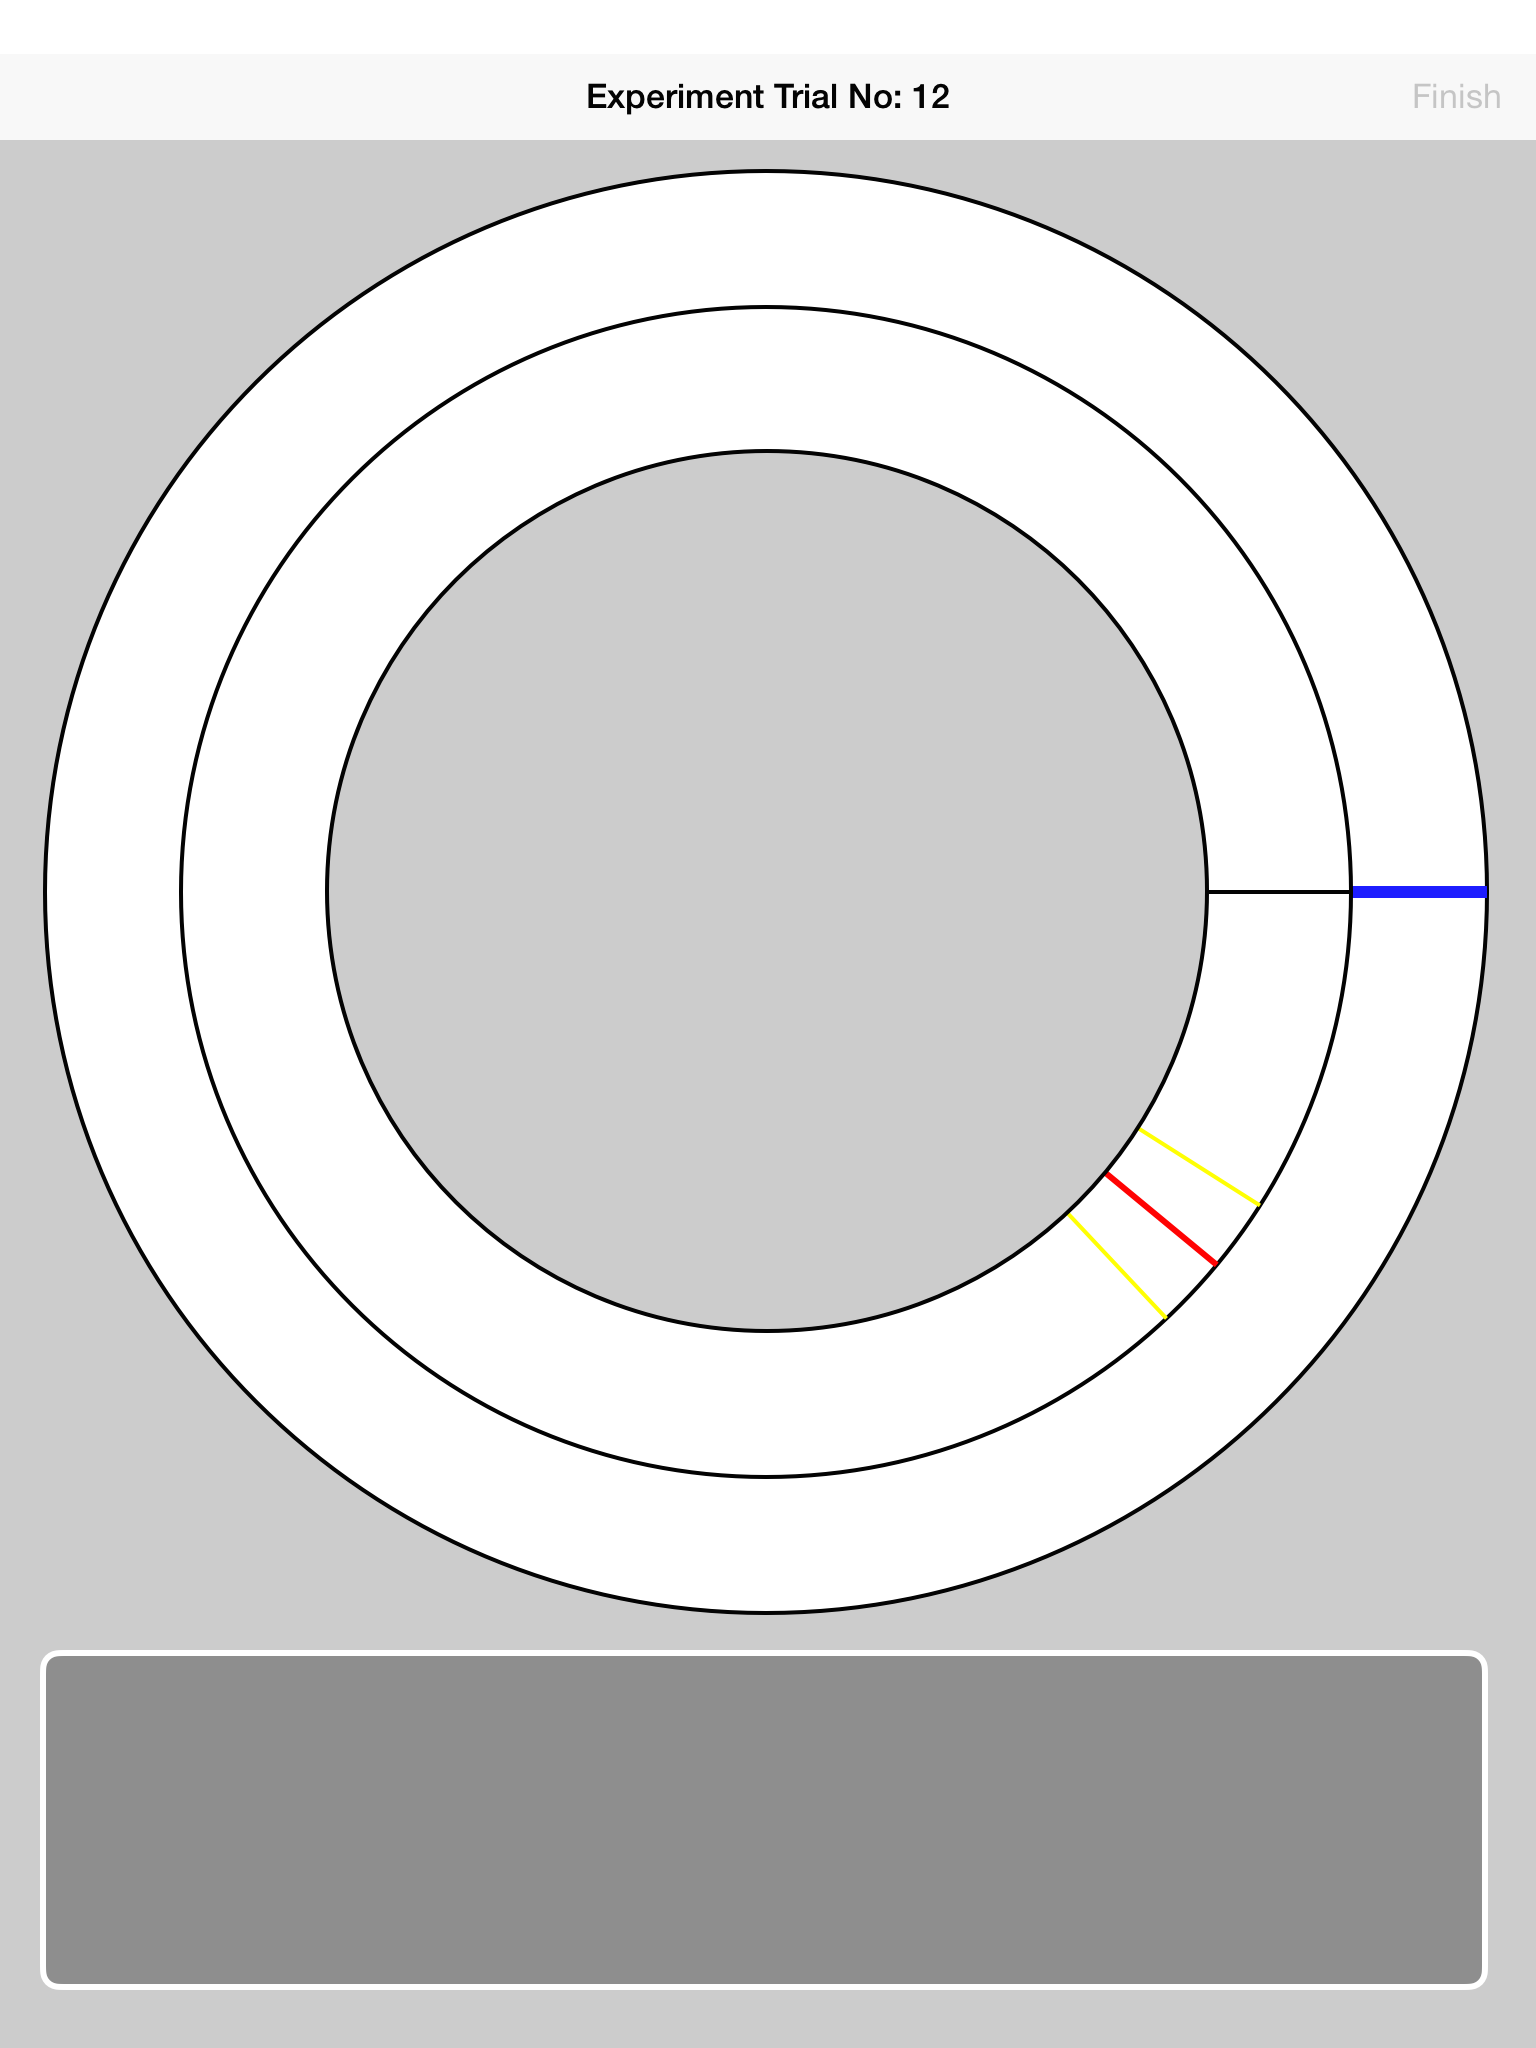
\includegraphics[scale=0.07]{figures/FND.png}
\caption{Feedback \& Continuous Targeting Interface}
\label{fig:FND}
\end{figure}

%%%%%%%%%%%%%%%%%%%%%
%%%%%%%%%%%%%%%%%%%%%
%%%%%%%%%%%%%%%%%%%%%
\subsection{No Feedback \& Discrete Targeting}

The rules for \emph{Discrete} targets apply and here. Thus, Region 2 (Figure \ref{fig:FFBasicTrialInterface}) is separated in $N$ buckets, all with equal size. Variable $N$ mostly specifies the difficulty of the trials. The target is the one coloured in red, and all others are inactive and coloured in gray. This category differs from the aforementioned because it is of type \emph{No Feedback}. That means that Region 3 (Figure \ref{fig:FFBasicTrialInterface}) does not exist. So, in the beginning we encounter the interface illustrated in Figure \ref{fig:NFD}. Our task  is to \textbf{a}) touch the screen, \textbf{b}) predict the contact area needed to select the target and \textbf{c}), confirm selection with QuickRelease. After confirming selection, we face the \textbf{Confirming Interface} shown in Figure \ref{fig:NFDConfirm}, in which we can observe our performance in the trials. Did we hit that target or not? This input can be used as a learning parameter which will help us to improve our performance as we move through the trials.

\begin{figure}[H]
\centering
\begin{subfigure}[b]{0.3\textwidth}
	\centering
	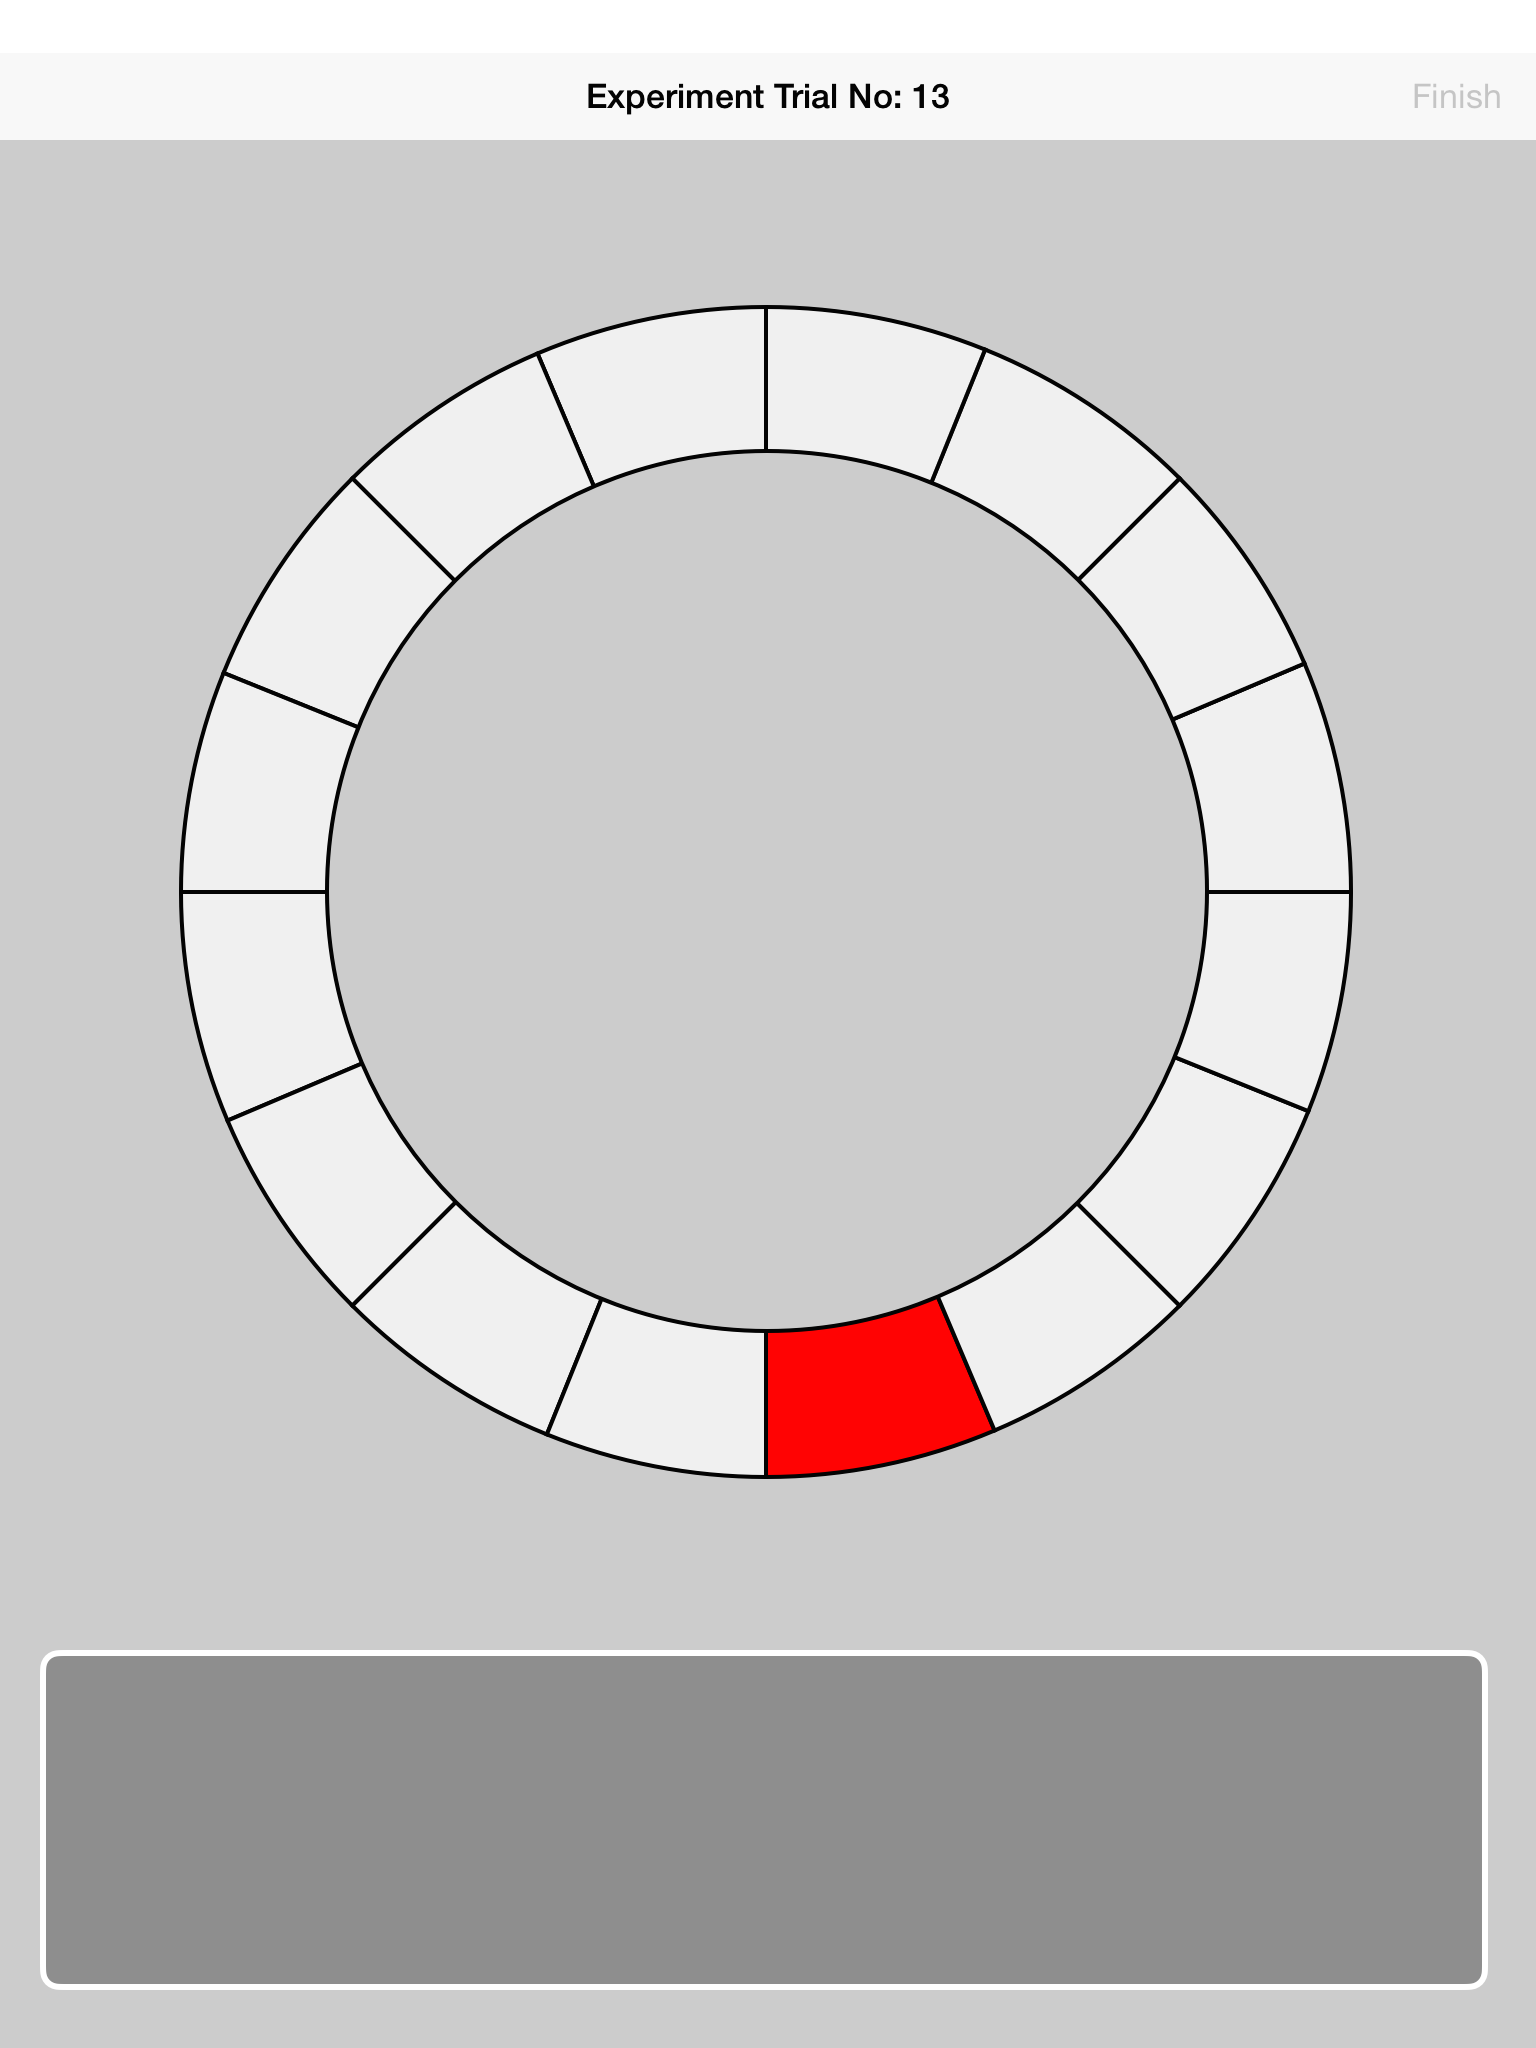
\includegraphics[width=\textwidth]{figures/NFD.png}
	\caption{Targeting Interface}
	\label{fig:NFD}
\end{subfigure}
\hfill
\begin{subfigure}[b]{0.3\textwidth}
	\centering
	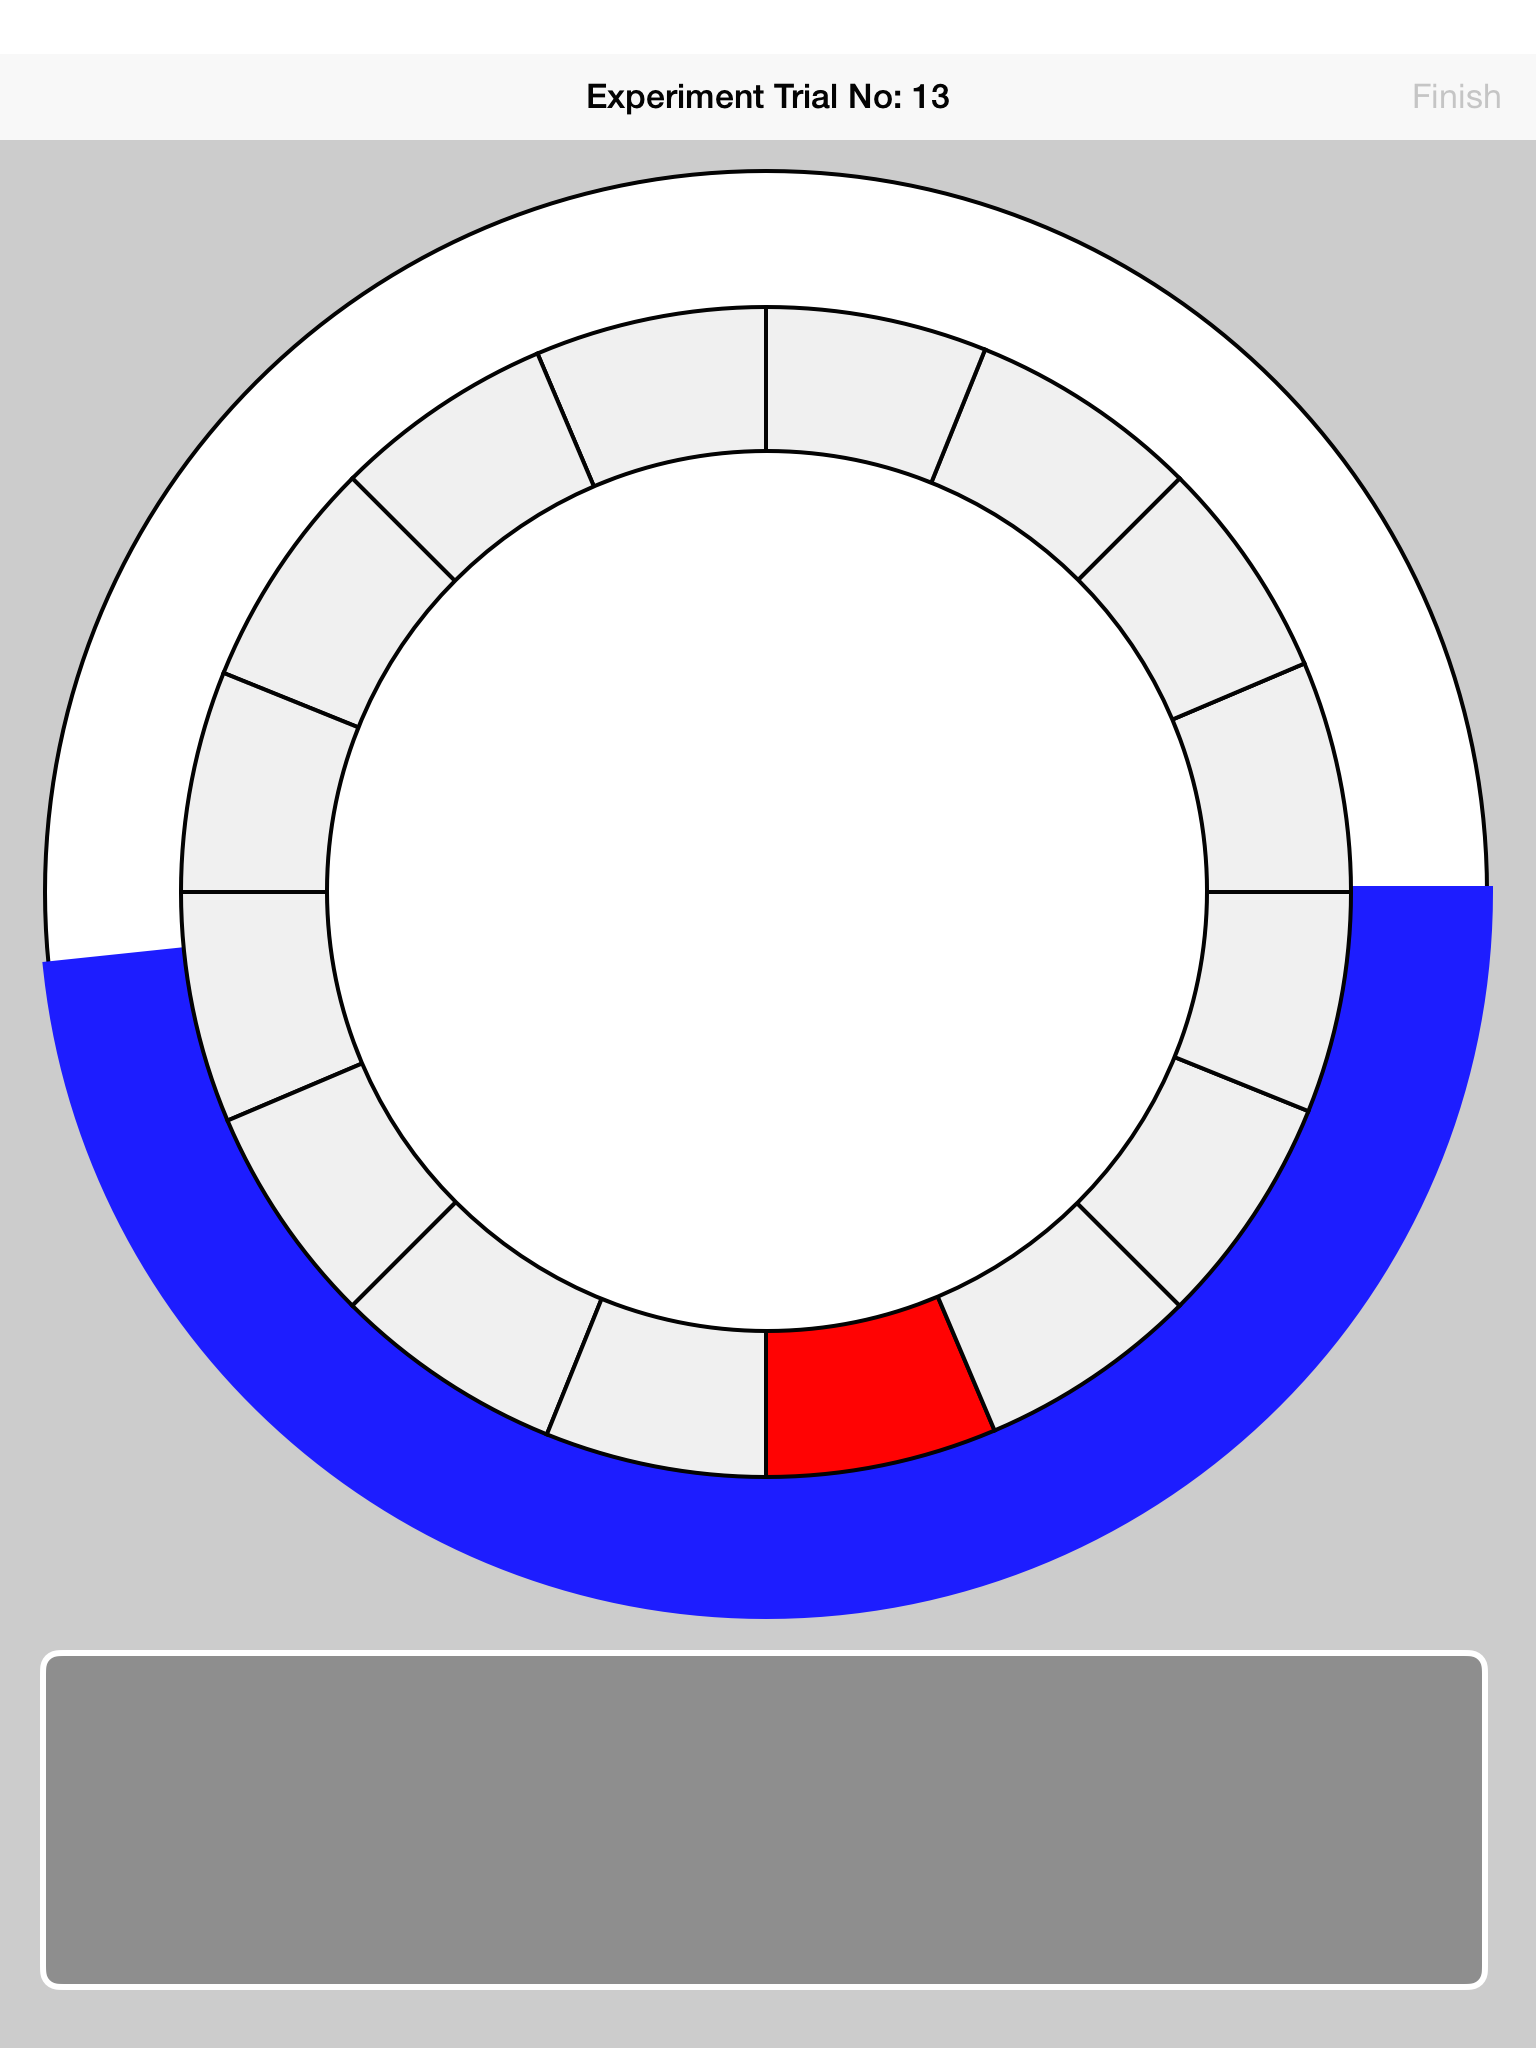
\includegraphics[width=\textwidth]{figures/NFDConfirm.png}
	\caption{Confirmation Interface}
	\label{fig:NFDConfirm}
\end{subfigure}
\caption{No Feedback \& Discrete Targeting and Confirmation Interface}
\label{fig:NFDGraph}
\end{figure}

%%%%%%%%%%%%%%%%%%%%%
%%%%%%%%%%%%%%%%%%%%%
%%%%%%%%%%%%%%%%%%%%%
\subsection{No Feedback \& Continuous Targeting}

\begin{figure}[H]
\centering
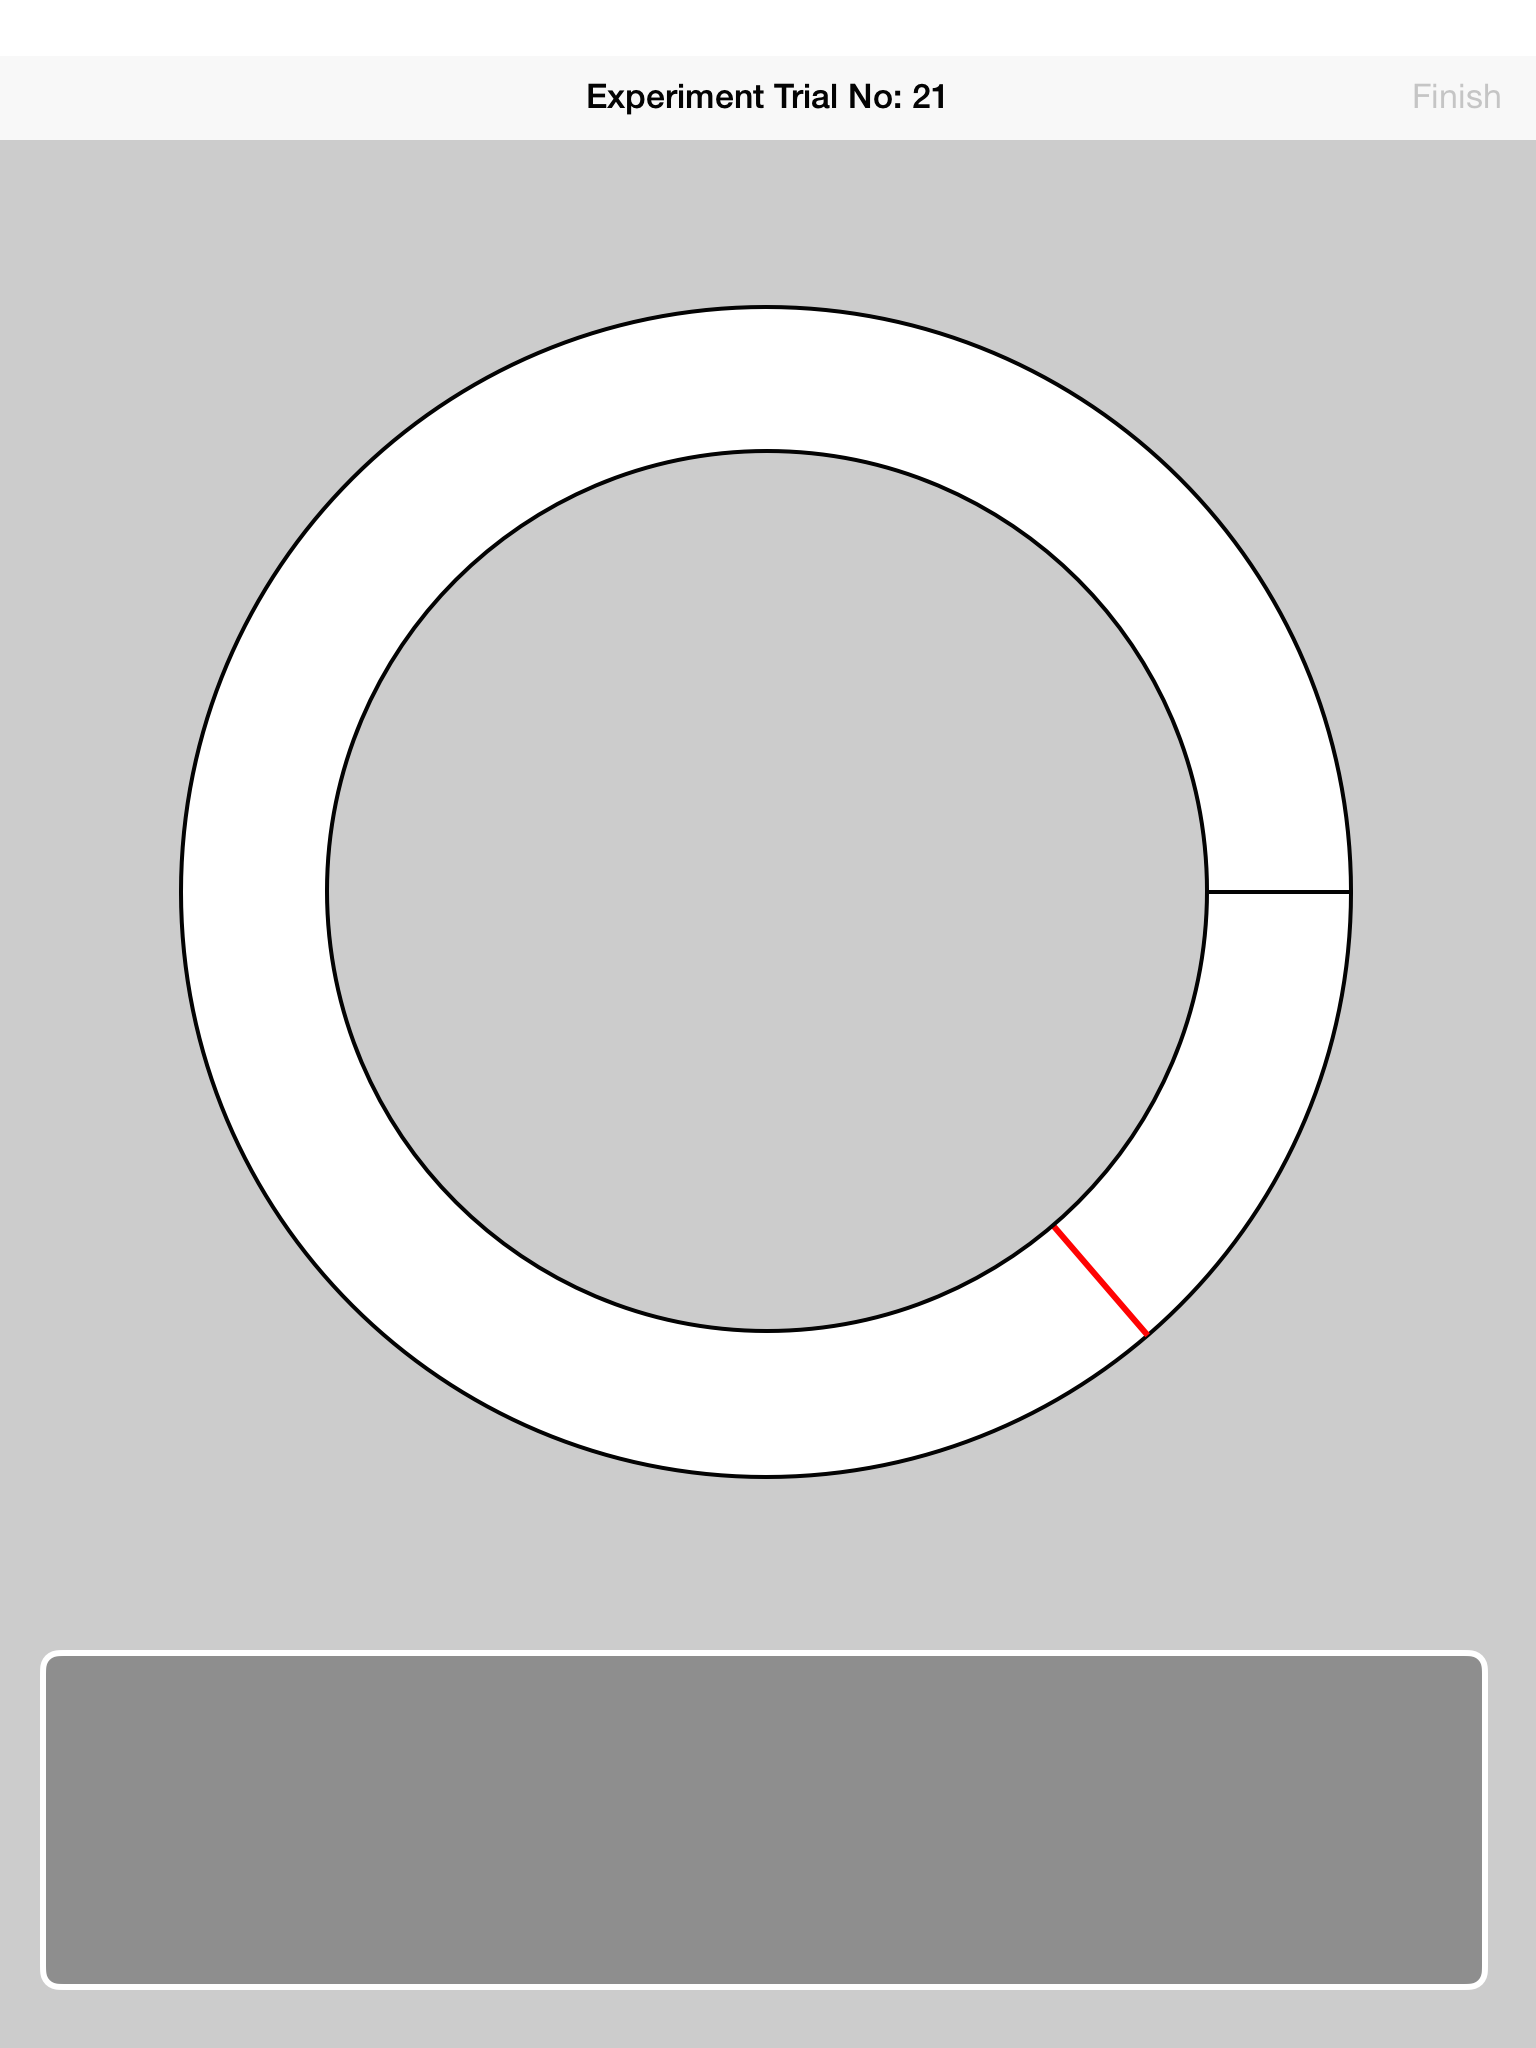
\includegraphics[scale=0.07]{figures/NFND.png}
\caption{No Feedback \& Continuous Targeting Interface}
\label{fig:NFND}
\end{figure}

Figure \ref{fig:NFND} presents the interface of the \emph{No Feedback \& Continuous Targeting} category. Targets are \emph{Continuous}, meaning that only one thin red line exist in Region 2 (Figure \ref{fig:FFBasicTrialInterface}). The two yellow lines, surrounding the red one still exist. They represent the offset limits and their distance is the offset range. It also of type \emph{No Feedback}. Thus, Region 3 (Figure \ref{fig:FFBasicTrialInterface}) does not exist. Our task is again to \textbf{a}) touch the screen, \textbf{b}) predict the contact area needed to select the target and \textbf{c}), confirm selection by lifting the finger form the screen. After confirming selection, we once more face the \textbf{Confirming Interface} shown in Figure \ref{fig:NFDConfirm}, in which we can observe our performance in the trials. 



%%%%%%%%%%%%%%%%%%%%%%%%%%%%%
%%%%%%%%%%%%%%%%%%%%%%%%%%%%%
%%%%%%%%%%%%%%%%%%%%%%%%%%%%%
%%%%%%%%%%%%%%%%%%%%%%%%%%%%%
%%%%%%%%%%%%%%%%%%%%%%%%%%%%%
%%%%%%%%%%%%%%%%%%%%%%%%%%%%%
\section{Final Sequence of Trials}
\label{sec:FinalSequenceofTrials}

% Explain   the   repetitions,   randomization,   and   generally   how   the   sequence   of each experiment is calculated.

Thus far we have explained all the main characteristics of our experiment. Now we should focus on the final sequence of the trials and the whole structure of the experiment. In this experiment we want to investigate 7 different N's, or bucket sizes, which can have the following values:

N = [2,3,4,6,8,12,16]

For each N we have the same amount of related targets. For instance if $N=2$, then we have two available targets, one for each bucket. If $N=4$, the we have 4 possible targets, etc.
As a result for all the above mentioned values for N we can gave the following number of possible targets:

$2(N=2)+3(N=3)+4(N=4)+6(N=6)+8(N=8)+12(N=12)+16(N=16) = 51 targets$

Then we have 4 different types of Trials: Feedback \& Discrete, No Feedback \& Discrete, Feedback \& Continuous, No Feedback \& Continuous.

For each of the above categories we conduct all the aforementioned targets. So the total number of Trials is:
$51*4 = 204$. Furthermore we need to randomize their order just to make sure that it will not have any effect in our study. After the randomization takes place we say that we have 1 \textbf{Repetition} of the Trials. Figure \ref{fig:ffRepetition} graphically illustrates this procedure.


\begin{figure}[h]
\centering
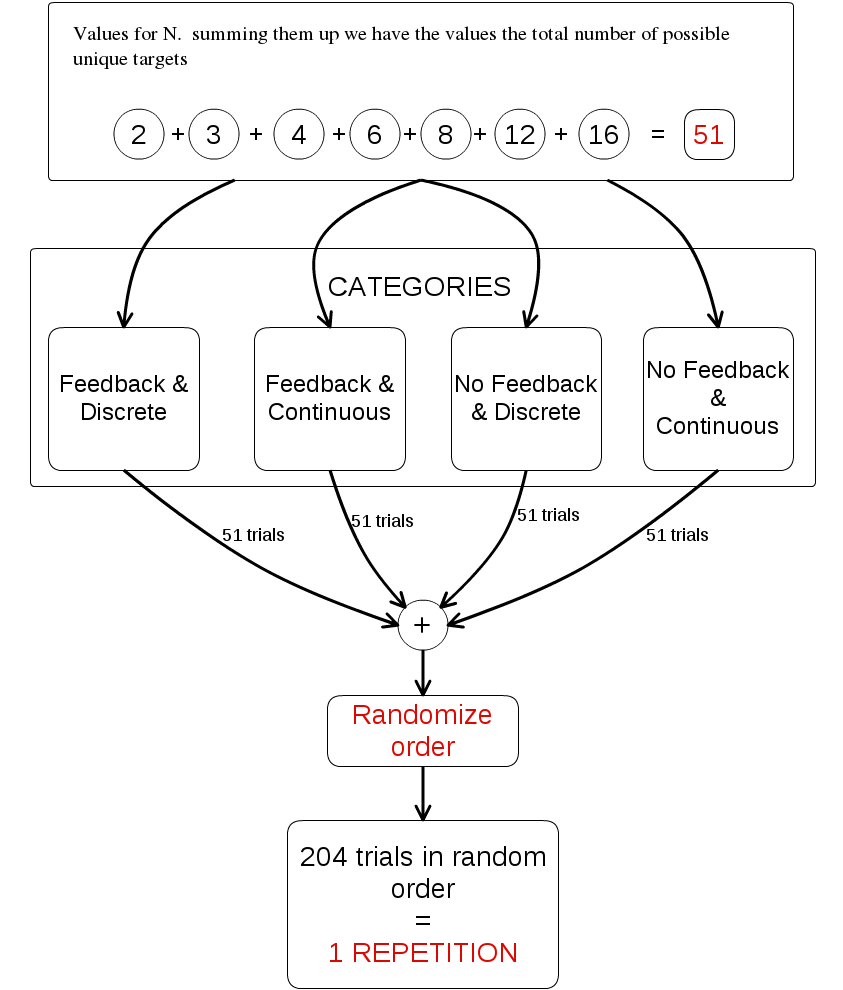
\includegraphics[width=0.6\textwidth]{figures/repetition.png}
\caption{Repetition Calculation}
\label{fig:ffRepetition}
\end{figure}


However, this experiment contains 3 repetitions of those trials and not only 1. So in total we will have $203*3repetitions = 612 trials$. We chose to have 3 Repetitions for the following 2 main reasons. 

\begin{itemize}
	\item There is no warm-up session for this experiment. Instead of having separate trials to train users, we chose to combine the Learning phase with the 1st repetition of the Trials. That way we will be able to observe and study the pace with which users and are learning this new interaction technique.

	\item The experiment should last enough so as to give users the time to absorb the information given, familiarize with the environment and technique and also explore whether side effects as distraction of attention and fatigue have an impact on their performance.
\end{itemize}

Figure \ref{fig:ffRepetition} graphically illustrates how the repetitions are combined together. It also gives an overview of the work-flow of Fat Finger.

\begin{figure}[h]
\centering
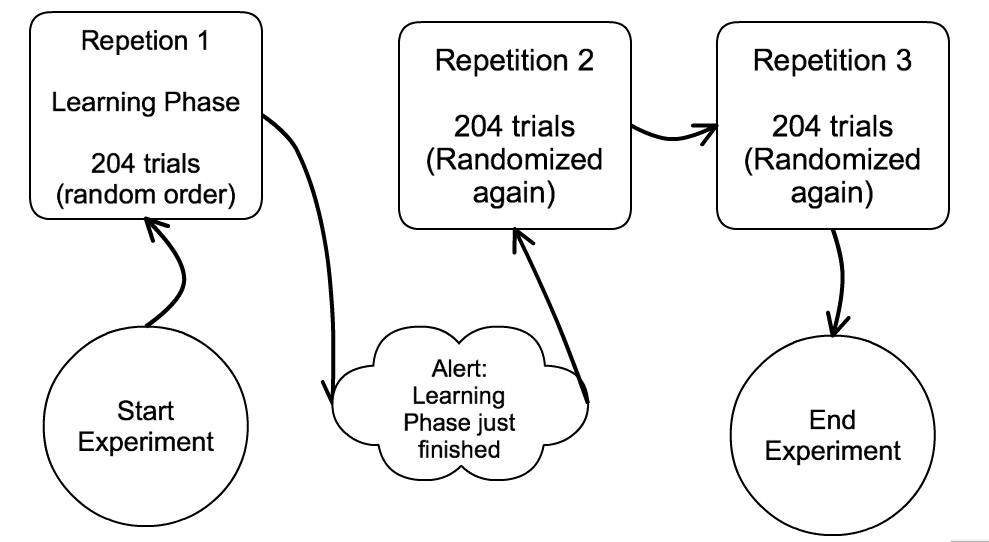
\includegraphics[width=0.6\textwidth]{figures/ffRepetitions.png}
\caption{Fat finger - Generalized experiment flow of repetitions}
\label{fig:ffRepetitions}
\end{figure}

Finally it should be mentioned that between each trial of this application there exist a button that should be pressed in order to proceed to the next trial. It is annotated with the text: "Next Trial" and the reason it exists is just for allowing users to take smalls breaks whenever needed. While this button is visible, no counter or other mechanisms are fired. Finally it has the same shape, size and position as Region 1 in Figure \ref{fig:FFBasicTrialInterface}


%%%%%%%%%%%%%%%%%%%%%%%%%%%%%
%%%%%%%%%%%%%%%%%%%%%%%%%%%%%
%%%%%%%%%%%%%%%%%%%%%%%%%%%%%
%%%%%%%%%%%%%%%%%%%%%%%%%%%%%
%%%%%%%%%%%%%%%%%%%%%%%%%%%%%
%%%%%%%%%%%%%%%%%%%%%%%%%%%%%
\section{Data Manipulation}

Data Monitoring and Exporting are of significant importance when we have to deal with the accomplishment of an experiment. When performing a user study you need to decide which parameters you are going to monitor, and to find a way to measure them. Code-wise, you need to implement a software that is able to calculate all the metrics you want to observe, and then store them somewhere consistently. After the experiment is finished, it is truly crucial to be able to export those data from the place they are stored into a common format that is accessible from another program. Summarizing we have a three-step process when we conduct an experiment. 

\begin{enumerate}
	\item Decide which parameters to measure.
	\item Store the observed values in a consistent database.
	\item Export the data to appropriate format (.xls, .csv, etc.)
\end{enumerate}

Our approach for the first two points is analyzed on section \ref{sec:monitoring}, while for the latter one on section \ref{sec:exporting}.
%%%%%%%%
%%%%%%%%
%%%%%%%%
%%%%%%%%
%%%%%%%%
\subsection{Monitoring}
\label{sec:monitoring}

Table \ref{tab:ffUniData} presents the basic parameters we measure that are common for all types of trials. The first column contains the name of the corresponding variable, the second a short description of its usage, and on the third we can observe which is the field of values for each variable.

%%%%
%% Universal Parameters
%%%%

\begin{table}[H]
\centering
\begin{tabular}{l || l || l}
Name & Description & Field of Values\\
\hline \hline
\textbf{trialID} & Incremental id of this trial & [1, 2, ..., 612] \\
\textbf{typeID} & Id of the type of the trial & [1,2,3,4] \\
\textbf{N} & Total number of Buckets & [2,3,4,6,8,12,16] \\
\textbf{min} & Minimum calibrated radius & $Float > 0$ \\
\textbf{max} & Maximum calibrated radius & $Float > 0$ \\
\textbf{rawInputValue} & Raw Value between Min and Max & Float number \\
\textbf{reEntries} & Number of Target Re-entries & $Decimal >= 0$ \\
\textbf{repetitionID} & Repetition id they belong to & [1,2,3] \\
\textbf{reTouches} & Number of Target Re-Touches & $Decimal >= 0$ \\
\textbf{target} & Which of the buckets was the target  & [1,2,...,n]\\
\textbf{totalTime} & Total time to accomplish the Trial & Float number
\end{tabular}
\caption{Fat Finger - Universal Parameters Monitored}
\label{tab:ffUniData}
\end{table}

Combining the above values, apart from giving us the possibility to uniquely identify the trials of the experiment, we can also reconstruct the whole experiment. This can be achieved, because we are storing the outcome of each trials, the rawData we collected form the user, the total time, etc. Now, we should further analyse each of those parameters:

\begin{itemize}
	\item \textbf{trialID}. Unique, auto-incremented identifier for each trial. Most importantly it specifies the order of appearance of the experiments. 

	\item \textbf{N}. Specifies the number of buckets. \textbf{N} is an indicator that is related, at least in the Feedback trials, with the difficulty. This study is mainly concerned in specifying an upper limit for the number of identifiable levels in the contact area range. Thus, N is the sorting parameter for being able to distinguish the upper limit for those levels. 
	
	\item \textbf{min}. The minimum value for the PathMajorRadius we collected from the calibration. During the calibration process, user can calibrate his finger as many times as he want. When he proceeds to the experiment, we collect the lastly calibrated values and store them accordingly.
	
	\item \textbf{max}. The same applies here too, except that we are referring to the maximum value of the PathMajorRadius.  
	
	\item \textbf{rawInputValue}. This is the PathMajorRadius value, for the contact area that hit the target. For Feedback trials, it is the last touch input size exactly after the 1 second delay has passed. For No feedback, it is the area just before lifting our finger.
	
	\item \textbf{reEntries}. Counts the times we went outside the target region. It starts counting after the initial entry to the target.
	
	\item \textbf{repetitionID}. Identifies in which of the three repetitions this trial belongs to.  
	
	\item \textbf{reTouches}. Counts the times we lifted our finger off the screen. Of course for \emph{No Feedback} trials this parameter is always zero since we confirm target selection by lifting our finger from the screen.
	
	\item \textbf{target}. Specifies which of the buckets is the target. Thus it can take values from 1 to N.
	
	\item \textbf{totalTime} Total completion time of the trial. The timer fires when the first touch is performed and stops when the confirming sound is being played. As a result \emph{Feedback} trials will have values $>=$ 1 second. This is because one second is the duration  someone has to be inside the target region to confirm target selection. On the other hand, on \emph{No feedback} trials, durations are generally shorter.
\end{itemize}



The above parameters are measured for all 4 types of trials. However, all except for \emph{Feedback\& Discrete} required some extra monitoring. \textbf{Feedback \& Continuous} has the following two extra measured parameters that are also presented in Table \ref{tab:ffFNDData}:

\begin{itemize}
	\item \textbf{targetPosition}. Defines the exact position of the Target. In this type, target is represented as a thin red line. The position will always be inside the \textbf{target}-th bucket out of the \textbf{n} in total. However since it is randomly positioned inside this bucket, we needed to record its accurate position. Value monitored is between \textbf{min} and \textbf{max}. To transform the position into circle degrees we can use the type $PositionInDegrees = \frac{targetPosition-min}{max-min}360$.
	\item \textbf{offset} Indicates how far we were from the target. It can be thought as an error rate too. The higher the offset the higher the error we performed on our selection. Positive values mean that we hit somewhere after the target. Negative values mean that we hit before it. Also offset is measured in percentage. If we want to find how many degrees we were off the target then we can just use the type: $DegreesOff = offset*360$
\end{itemize}

%%%%
%% Feedback Continuous Parameters
%%%%

\begin{table}[H]
\centering
\begin{tabular}{l || l || l}
Name & Description & Field of Values \\
\hline \hline
\textbf{targetPosition} & Position of the Target & \textbf{min}$<=$Float$<=$\textbf{max} \\
\textbf{offset} & Distance from target in percentage & float :[-1 to +1] 
\end{tabular}
\caption{Fat Finger - Feedback \& Continuous Targeting additional parameters monitored}
\label{tab:ffFNDData}
\end{table}


\textbf{No Feedback \& Discrete} targeting requires a different set of extra parameters to be measured. Feedback region does not exist in this type, which means that users have to predict where it is. This type of trial requires longer learning time. Thus for the initial trials we expect that participants predictions will not be very accurate. As a result, offset will be high. To monitor that we use the following two parameters as shown in Table \ref{tab:ffNFDData}:
\begin{itemize}
	\item \textbf{hitInsideTarget} As it can be inferred form its name, it indicates whether we actually hit inside the target or outside. 
	\item \textbf{offset} mostly represents the error in percentage over the whole range. In \emph{No Feedback} trials error can be extremely high as there is no limitation in performing in-target selection. Thus positive values mean that the selection was performed at a point after the center of the target, while negative values stand for before.
\end{itemize}


%%%%
%% No Feedback Discrete Parameters
%%%%
\begin{table}[H]
\centering
\begin{tabular}{l || l || l}
Name & Description & Field of Values  \\
\hline \hline
\textbf{offset} & Distance from target in percentage & float :[-1 to +1] \\
\textbf{hitInsideTarget} & Indicates if we successfully hit the Target & True, False
\end{tabular}
\caption{Fat Finger - No Feedback \& Discrete Targeting additional parameters monitored}
\label{tab:ffNFDData}
\end{table}

Finally, in \textbf{No Feedback \& Continuous Targeting} we meet a combination of the extra parameters we have already mentioned. To better monitor this type we use the extra supplementary parameters, illustrated in Table \ref{tab:ffNFNDData}. Each of them has been already explained and analyzed in the aforementioned types.


%%%%
%% No Feedback Continuous Parameters
%%%%

\begin{table}[H]
\centering
\begin{tabular}{l || l || l}
Name & Description & Field of Values \\
\hline \hline
\textbf{offset} & Distance from target in percentage & float :[-1 to +1] \\
\textbf{targetPosition} & Position of the Target & \textbf{min}$<=$Float$<=$\textbf{max} \\
\textbf{hitInsideTarget} & Indicates if we successfully hit the Target & True, False
\end{tabular}
\caption{Fat Finger - No Feedback \& Continuous Targeting additional parameters monitored}
\label{tab:ffNFNDData}
\end{table}

%%%%%%%%
%%%%%%%%
%%%%%%%%
%%%%%%%%
%%%%%%%%
\subsection{Exporting}
\label{sec:exporting}

Monitoring the results and saving them into a database was half the way towards the fulfilment of our goal. There is a need to export them into a reasonable format so that they can be imported into a statical analysis tool. Fat Finger used Core Data for storing all the aforementioned parameters.
\emph{"Core Data is an object graph and persistence framework provided by Apple. It allows data organized by the relational entity–attribute model to be serialized into XML, binary, or SQLite stores. The data can be manipulated using higher level objects representing entities and their relationships. Core Data manages the serialized version, providing object life-cycle and object graph management, including persistence. Core Data interfaces directly with SQLite, insulating the developer from the underlying SQL."} \cite{coreData}

Core Data does not provide a specific output data format, neither has an automatic exporting tool. However, since we have full access on the data stored in database we can implement our own customized export tool. For the purposes of this study, I used the Comma Separated Values (\textbf{.csv}) format. The output file has the following format:

\begin{itemize}
	\item Each line represents a case. In other words, each line represents the data collected for a specific trial of a user.
	\item Each case can be uniquely identified by the combination of the userID and trialID parameters.
	\item Each user performed 612 trials. Those he will be presented by 612 unique cases.
	\item Each variable (n, targets, userID, totalTime etc.) is represented by a column.
\end{itemize}






